\ifdefined\included
\else
\documentclass[a4paper,11pt,twoside]{StyleThese}
\usepackage{amsmath,amssymb}             % AMS Math
\usepackage[french]{babel}
\usepackage[utf8]{inputenc}
\usepackage[T1]{fontenc}
\usepackage{tabularx}
%\usepackage{tabular}
\usepackage{multirow}


\usepackage[tight,footnotesize]{subfigure}
\usepackage{algorithm} %To allow algorithm environment
\usepackage{algpseudocode} %Provides algorithmic environment

\usepackage{hhline}
\usepackage[left=1.5in,right=1.3in,top=1.1in,bottom=1.1in,includefoot,includehead,headheight=13.6pt]{geometry}
\renewcommand{\baselinestretch}{1.05}

% Table of contents for each chapter

\usepackage[nottoc, notlof, notlot]{tocbibind}
\usepackage[french]{minitoc}
\setcounter{minitocdepth}{2}
\mtcindent=15pt
% Use \minitoc where to put a table of contents

\usepackage{aecompl}

% Glossary / list of abbreviations

\usepackage[intoc]{nomencl}
\renewcommand{\nomname}{Liste des Abréviations}

\makenomenclature

% My pdf code

\usepackage{ifpdf}

\ifpdf
  \usepackage[pdftex]{graphicx}
  \DeclareGraphicsExtensions{.jpg}
  \usepackage[a4paper,pagebackref,hyperindex=true]{hyperref}
  \usepackage{tikz}
  \usetikzlibrary{arrows,shapes,calc}
\else
  \usepackage{graphicx}
  \DeclareGraphicsExtensions{.ps,.eps}
  \usepackage[a4paper,dvipdfm,pagebackref,hyperindex=true]{hyperref}
\fi

\graphicspath{{.}{images/}}

%nicer backref links
\renewcommand*{\backref}[1]{}
\renewcommand*{\backrefalt}[4]{%
\ifcase #1 %
(Non cité.)%
\or
(Cité en page~#2.)%
\else
(Cité en pages~#2.)%
\fi}
\renewcommand*{\backrefsep}{, }
\renewcommand*{\backreftwosep}{ et~}
\renewcommand*{\backreflastsep}{ et~}

% Links in pdf
\usepackage{color}
\definecolor{linkcol}{rgb}{0,0,0.4} 
\definecolor{citecol}{rgb}{0.5,0,0} 
\definecolor{linkcol}{rgb}{0,0,0} 
\definecolor{citecol}{rgb}{0,0,0}
% Change this to change the informations included in the pdf file

\hypersetup
{
bookmarksopen=true,
pdftitle="Évaluation de la sécurité des équipements grand public connectés à Internet",
pdfauthor="Yann BACHY", %auteur du document
pdfsubject="Thèse", %sujet du document
%pdftoolbar=false, %barre d'outils non visible
pdfmenubar=true, %barre de menu visible
pdfhighlight=/O, %effet d'un clic sur un lien hypertexte
colorlinks=true, %couleurs sur les liens hypertextes
pdfpagemode=None, %aucun mode de page
pdfpagelayout=SinglePage, %ouverture en simple page
pdffitwindow=true, %pages ouvertes entierement dans toute la fenetre
linkcolor=linkcol, %couleur des liens hypertextes internes
citecolor=citecol, %couleur des liens pour les citations
urlcolor=linkcol %couleur des liens pour les url
}

% definitions.
% -------------------

\setcounter{secnumdepth}{3}
\setcounter{tocdepth}{2}

% Some useful commands and shortcut for maths:  partial derivative and stuff

\newcommand{\pd}[2]{\frac{\partial #1}{\partial #2}}
\def\abs{\operatorname{abs}}
\def\argmax{\operatornamewithlimits{arg\,max}}
\def\argmin{\operatornamewithlimits{arg\,min}}
\def\diag{\operatorname{Diag}}
\newcommand{\eqRef}[1]{(\ref{#1})}

\usepackage{rotating}                    % Sideways of figures & tables
%\usepackage{bibunits}
%\usepackage[sectionbib]{chapterbib}          % Cross-reference package (Natural BiB)
%\usepackage{natbib}                  % Put References at the end of each chapter
                                         % Do not put 'sectionbib' option here.
                                         % Sectionbib option in 'natbib' will do.
\usepackage{fancyhdr}                    % Fancy Header and Footer

% \usepackage{txfonts}                     % Public Times New Roman text & math font
  
%%% Fancy Header %%%%%%%%%%%%%%%%%%%%%%%%%%%%%%%%%%%%%%%%%%%%%%%%%%%%%%%%%%%%%%%%%%
% Fancy Header Style Options

\pagestyle{fancy}                       % Sets fancy header and footer
\fancyfoot{}                            % Delete current footer settings

%\renewcommand{\chaptermark}[1]{         % Lower Case Chapter marker style
%  \markboth{\chaptername\ \thechapter.\ #1}}{}} %

%\renewcommand{\sectionmark}[1]{         % Lower case Section marker style
%  \markright{\thesection.\ #1}}         %

\fancyhead[LE,RO]{\bfseries\thepage}    % Page number (boldface) in left on even
% pages and right on odd pages
\fancyhead[RE]{\bfseries\nouppercase{\leftmark}}      % Chapter in the right on even pages
\fancyhead[LO]{\bfseries\nouppercase{\rightmark}}     % Section in the left on odd pages

\let\headruleORIG\headrule
\renewcommand{\headrule}{\color{black} \headruleORIG}
\renewcommand{\headrulewidth}{1.0pt}
\usepackage{colortbl}
\arrayrulecolor{black}

\fancypagestyle{plain}{
  \fancyhead{}
  \fancyfoot{}
  \renewcommand{\headrulewidth}{0pt}
}

%\usepackage{MyAlgorithm}
%\usepackage[noend]{MyAlgorithmic}
\usepackage[ED=MITT - STICIA, Ets=INP]{tlsflyleaf}
%%% Clear Header %%%%%%%%%%%%%%%%%%%%%%%%%%%%%%%%%%%%%%%%%%%%%%%%%%%%%%%%%%%%%%%%%%
% Clear Header Style on the Last Empty Odd pages
\makeatletter

\def\cleardoublepage{\clearpage\if@twoside \ifodd\c@page\else%
  \hbox{}%
  \thispagestyle{empty}%              % Empty header styles
  \newpage%
  \if@twocolumn\hbox{}\newpage\fi\fi\fi}

\makeatother
 
%%%%%%%%%%%%%%%%%%%%%%%%%%%%%%%%%%%%%%%%%%%%%%%%%%%%%%%%%%%%%%%%%%%%%%%%%%%%%%% 
% Prints your review date and 'Draft Version' (From Josullvn, CS, CMU)
\newcommand{\reviewtimetoday}[2]{\special{!userdict begin
    /bop-hook{gsave 20 710 translate 45 rotate 0.8 setgray
      /Times-Roman findfont 12 scalefont setfont 0 0   moveto (#1) show
      0 -12 moveto (#2) show grestore}def end}}
% You can turn on or off this option.
% \reviewtimetoday{\today}{Draft Version}
%%%%%%%%%%%%%%%%%%%%%%%%%%%%%%%%%%%%%%%%%%%%%%%%%%%%%%%%%%%%%%%%%%%%%%%%%%%%%%% 

\newenvironment{maxime}[1]
{
\vspace*{0cm}
\hfill
\begin{minipage}{0.5\textwidth}%
%\rule[0.5ex]{\textwidth}{0.1mm}\\%
\hrulefill $\:$ {\bf #1}\\
%\vspace*{-0.25cm}
\it 
}%
{%

\hrulefill
\vspace*{0.5cm}%
\end{minipage}
}

\let\minitocORIG\minitoc
\renewcommand{\minitoc}{\minitocORIG \vspace{1.5em}}

\usepackage{multirow}
%\usepackage{slashbox}

\newenvironment{bulletList}%
{ \begin{list}%
	{$\bullet$}%
	{\setlength{\labelwidth}{25pt}%
	 \setlength{\leftmargin}{30pt}%
	 \setlength{\itemsep}{\parsep}}}%
{ \end{list} }

\newtheorem{definition}{Définition}
\renewcommand{\epsilon}{\varepsilon}

% centered page environment

\newenvironment{vcenterpage}
{\newpage\vspace*{\fill}\thispagestyle{empty}\renewcommand{\headrulewidth}{0pt}}
{\vspace*{\fill}}

\usepackage{tablefootnote}
\sloppy
\begin{document}
\setcounter{chapter}{0} %% Numéro du chapitre précédent ;)
\dominitoc
\faketableofcontents
\fi

\chapter{Introduction}
%\addstarredchapter{Introduction}
\minitoc

\section{Contexte général}
%global intro
De nombreux fantasmes ont toujours entouré la représentation que l'on se fait des robots. Le concept de créatures intelligentes confectionnées par la main de l'homme est déjà présent dans les mythologies tel que le mythe du Golem dans la mythologie juive ou l'histoire de Pygmalion et Galatée dans la mythologie grecque, ou encore les servantes androïdes en or du dieu Héphaïstos que l'on retrouve dans \textit{l'Illiade} d'Homère.

On retrouve dans la littérature du XIXe siècle le thème de l'automate prenant vie, à travers des œuvres telles que \textit{L'homme au sable} d'Ernst Theodor Amadeus Hoffmann ou le compte de fées \textit{Pinocchio} de Carlo Collodi. C'est également à cette époque qu'est paru le célèbre roman de Mary Shelley: \textit{Frankenstein ou le Prométhée moderne}. Cette œuvre met en scène la perte de contrôle du savant Frankenstein sur sa créature, cette dernière se révolte contre son créateur et les êtres humains en général dont il est rejeté. 

Cette thématique de révolte contre l'homme sera très largement reprise dans les œuvres de science-fiction occidentales du XXè siècle. Un auteur cependant se démarque de cette ligne en présentant un recueil de nouvel nommé \textit{Les Robots}. Il s'agit de l'auteur américain Isaac Asimov, qui à travers ces nouvelles présente les limites possibles de système robotique et comment s'assurer que les robots s'évertuent à contribuer au bien-être des humains en énonçant notamment les trois lois de la robotique. Ces lois, implantées au cœur même du système robotique, doivent forcer le robot à agir pour garantir l'intégrité physique de tout être humain, pour obéir aux ordres des hommes et enfin pour garantir sa propre intégrité physique.

De nos jours, la thématique de la machine échappant au contrôle de l'homme est toujours présente notamment dans le cinéma Hollywoodien à travers les œuvres telles que Terminator, \textit{The Machine} ou encore \textit{Ex-Machina}. Il est cependant à constater que ces machines ont des comportements de plus en plus proches de l'être humain.  de par leur intelligence mais aussi leur capacités d'établir des interactions sociales  avec l'homme.
Certaines œuvres cependant, dans la lignée d'Asimov, décrivent les robots comme des compagnons particulièrement utiles et dociles, tel que le Pinocchio moderne David du film \textit{AI} ou le robot médical Baymax du film d'animation \textit{les nouveaux héros}.

La représentation que l'opinion publique se fait des robots a son importance car elle influence la perception des robots \cite{Sundar2016} et donc la direction donnée à la recherche. Ainsi, la culture japonaise est décrite comme robophile \cite{gilson98}. Dans ce même pays, on constate un investissement massif dans la recherche en robotique, notamment dans la robotique de service depuis plusieurs décennies.

Malgré les scénarios apocalyptiques de certaines œuvres et les angoisses sociétales liées au robot, tel la suppression d’emplois peu qualifiés, les robots sont entrés dans nos usines et commencent à arriver dans nos maisons. Les premiers modèles ont pris la forme d'automates programmables dans les industries et de robots aspirateurs ou de jouets dans les foyers. Ces premières formes ont une intelligence très limitée et liée à une tâche, le plus souvent assez basique, à accomplir. Ces premiers modèles, de par leur adaptabilité très limitée et leur intelligence qui tient plus de la réaction que du raisonnement, sont plus proches de l'automate que  de réelles systèmes intelligents. Cependant, on constate depuis quelques années une complexification des robots industriels et domestiques. Cette complexification permet aux robots les plus récents de prendre en compte l'homme. Ainsi, l'homme et la machine vont être amenés de plus en plus à se côtoyer, que se soit sur le lieu de travail avec des robot coéquipiers ou dans les foyers avec les robots assistants. C'est dans ce contexte que les robots sociaux arrivent sur le marché.
Ainsi, dès le début des années 2000, des robots ayant pour but d'interagir avec l'homme sont commercialisés par Sony: tout d'abord Aibo\footnote{https://fr.wikipedia.org/wiki/Aibo} qui prends la forme d'un chien puis Qrio\footnote{https://fr.wikipedia.org/wiki/Qrio}, un petit robot humanoïde. Dans la même lignée que Qrio, Aldebaran (aujourd'hui devenu Softbank Robotics) sort fin 2006 le robot NAO\footnote{https://www.ald.softbankrobotics.com/fr/cool-robots/nao} qui deviendra rapidement une plateforme très utilisée dans les laboratoires de recherches et universités à travers le monde.
Plus récemment, Softbank Robotics a également mis au point le robot humanoïde Pepper\footnote{https://www.ald.softbankrobotics.com/fr/cool-robots/pepper} qui est déjà utilisé comme plateforme de renseignements et d'informations commerciales. 
Il est également à constater que plusieurs campagnes de crowd-founding ont rencontré un franc succès pour des projets de plateformes robotiques sociales pour le domicile. On peut notamment citer les robots Jibo\footnote{https://www.jibo.com/} ou Buddy\footnote{http://www.bluefrogrobotics.com/fr/buddy-fr/}. Ces deux projets de plateforme robotique interagissant avec l'homme et destinée au grand public, ont reçu des retours très positifs et sont révélateurs de l'engouement de la population pour ce genre de plateforme. En effet, le secteur de la robotique de service et domestique (robots assistants/équipiers) est considéré comme un des enjeux
économiques de ce siècle. On estime que d’ici à 2020, le marché de la robotique de service (tous secteurs confondus) pourrait représenter un volume supérieur à 15.69 milliards de dollars par an selon une étude de Grand View Research\footnote{http://www.grandviewresearch.com/industry-analysis/service-robotics-industry}. 

%Vieillissement de la population
L'un des intérêts premier de la robotique d'assistance est lié au vieillissement de la population. En effet, les robots autonomes d'assistance pourraient permettre de redonner une certaine autonomie aux personnes âgées ainsi qu'un accès aux technologies modernes à travers l'utilisation intuitive des robots comme interface.
Pour ce qui est des robots équipiers, ils pourraient permettre d'exécuter des tâches répétitives, pénibles, mais également des tâches dangereuses voir irréalisables par l'homme (par exemple celles nécessitant une grande précision) tout en travaillant en collaboration avec un opérateur humain. 

Cependant, pour le robot coéquipier comme pour le robot assistant, le contact avec l'homme rend important, si ce n'est nécessaire, d'incorporer une représentation de l'homme et des comportements sociaux pour interagir avec celui-ci. Le but n'étant pas de copier l'homme ou de le remplacer, mais uniquement de mettre en place des mécanismes permettant une interaction efficace, agréable et intuitive pour l'homme. Pour cela le robot doit être capable d'estimer la situation et l'état de l'homme et exhiber des comportements pouvant être compris par l'homme. Dans cette thèse nous présenterons comment le robot peut créer et maintenir une représentation de l'environnent dans lequel il évolue ainsi que des individus avec lesquels il interagit, afin de pouvoir montrer des comportements socialement acceptables par l'homme. Ainsi, l'un des enjeux est de construire une sémantique liée au contexte de l'interaction afin d'interpréter correctement les actions physiques et les actes de paroles de l'homme ainsi que son intention afin de pouvoir aider l'homme au mieux tout en agissant et dialoguant de façon compréhensible et acceptable par celui-ci.

\section{Contexte de la thèse}
%Todo projet mardi, équipe ris, previous work...
% global architecture?

\subsection{Le projet MaRDi}
Cette thèse a été réalisée dans le cadre du projet MaRDi (MAn-Robot Dialogue)\footnote{http://mardi.metz.supelec.fr} de l’Agence Nationale pour la Recherche (ANR). Il a été financé par l’appel à projet Contenu et interactions.
Ce projet vise à étudier l’apport d’une approche "située" du dialogue Homme-
Robot. Le terme "situé" est ici relatif à l’incarnation physique d’un système de dialogue dans une plateforme robotique qui permet l’intégration d’informations issues de la perception du robot dans le contexte de l’interaction pour compléter ou lever des ambiguïtés introduites par le médium vocal. L’originalité de l’approche est de ne pas considérer les technologies vocales comme disponibles et dissociées de la tâche d’interaction Homme-Robot, mais bel et bien comme moyen d’en améliorer l’expérience et les performances.

\subsection{Environnement de travail}
\label{sec:workEnv}
Cette thèse a été réalisé au LAAS-CNRS dans l'équipe RIS (Robot InteractionS).
Elle s'inscrit dans la continuité de travaux précédemment réalisés par cette même équipe et contribue à l'architecture globale visant à construire un système robotique complet. Les problématiques abordées sont liées à l'interaction homme-robot, du raisonnement sur les données issues de la perception à la planification de mouvements en passant par la prise de décision et la planification de tâches.
%TODO: cite paper for each, or thesis?

Ainsi, l'architecture cognitive globale envisagée par notre équipe pour un robot d'interaction s'inspire de l'architecture en trois niveaux décrite dans \cite{pacherie2012phenomenology} concernant le suivi des actions jointes entre humains. Cette architecture consiste en un premier niveau appelé niveau distal partagé (\textit{Shared Distal level}) qui s'occupe des problèmes liés à l'intention (engagement, élaboration et suivi d'un plan partagé). Un second niveau appelé niveau proximal partagé (\textit{Shared Proximal level}) qui s'occupe de l'execution des actions planifiées provenant du niveau distal à haut niveau. Enfin le dernier niveau appelé  intention motrice couplée (\textit{Coupled Motor intention}) qui assure la coordination au niveau de l'espace et du temps durant l'execution de l'action.
Basé sur cette architecture, Alami et al. proposent dans \cite{alami1998architecture} une architecture robotique avec trois niveaux. Cette architecture a par la suite été développée pour l'interaction Homme-Robot \cite{alami2011robot,alami2013human,fioreiser2014} afin d'intégrer des capacités de prise en compte de l'homme dans les différents niveaux. 
Basé sur ces travaux, nous avons présenté dans \cite{Devin16} les compétences qui nous semblent essentielles pour un robot interagissant avec l'homme ainsi que l'architecture cognitive qui permet de doter le robot de ces capacités.
Cette architecture est présentée à la figure \ref{fig:archiglobal}.



\begin{figure}[!t]
        \centering
          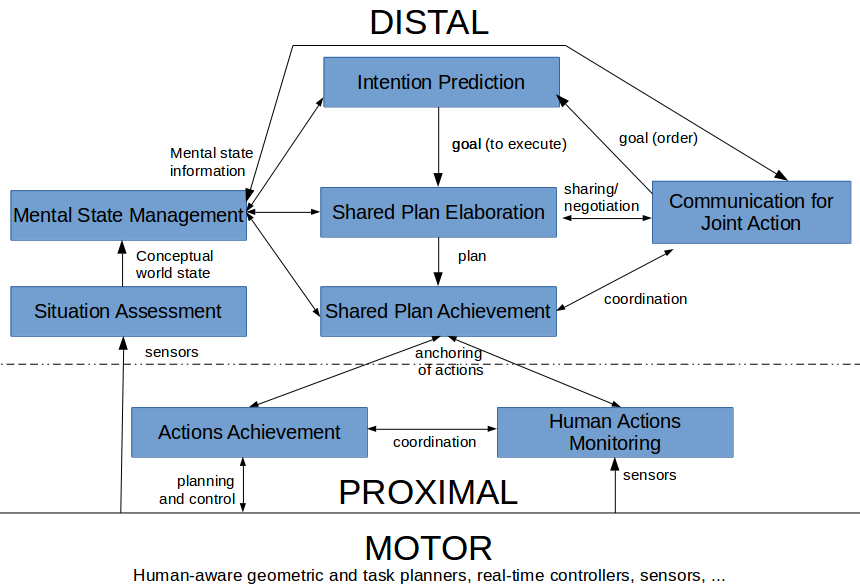
\includegraphics[width=0.99\textwidth]{img/cogarch.png}
    \caption{Architecture cognitive pour l'interaction homme-robot mise en place par l'équipe RIS du LAAS-CNRS.}
       \label{fig:archiglobal}
\end{figure}

\section{Motivations}
%Challenges
%Maybe start with a scenario?
%Big focus on HRI


\subsection{Scénario}

La robotique d'assistance et plus généralement la recherche concernant la conception et la confection de systèmes interagissant avec l'homme a encore de nombreux défis à relever. Pour exposer certains de ces défis, nous proposons un scénario d'illustration.

Imaginons un couple, Bob et Alice, vivant dans un appartement avec un robot d'assistance. Prenons la situation où Alice rentre du travail et décide de cuisiner une nouvelle recette avec l'aide de son robot. Avant de commencer la préparation, Alice demande à son robot de l'aider à réunir les ingrédients et ustensiles pour faire la recette.
Pour pouvoir aider efficacement Alice, le robot a donc besoin de capacités élémentaires telles que la navigation, la perception et la préhension d'objets.

Par exemple, Alice peut demander au robot d'apporter un objet qui est sur la table du salon. Pour comprendre Alice, à supposer que le robot soit capable de reconnaissance vocale, il lui faut comprendre également les concepts énoncés par Alice et les relier à la réalité du contexte situé. Ceci implique pour le robot de raisonner sur l'environnement afin de produire ce genre de relations spatiales (ici un objet \textit{"sur"} un autre). Ceci afin de comprendre et d'être compris de l'humain avec lequel il interagit.

Imaginons à présent qu'Alice ait besoin de son batteur à œufs qui est dans la commode du salon. Imaginons également que pendant la journée, Bob ait utiliser le batteur de la commode sans le ranger à son emplacement habituel, et que le robot ait perçu ce changement.
Un comportement utile et proactif pour le robot serait, en voyant Alice se déplacer vers la commode du salon, de la prévenir du changement de position du batteur.
Pour parvenir à cela, le robot doit être capable de se représenter les états de connaissances des humains qui l'entourent ainsi que d'interpréter leurs intentions en fonction du contexte (ici chercher les ustensiles pour réaliser une recette), de leur état mental (ici Alice pense que le batteur est dans la commode) et de leurs actions (Alice se dirige vers la commode du salon).

Une fois que les ustensiles et les ingrédients sont réunis, il reste à confectionner le plat. Imaginons qu'Alice demande au robot de la guider pour effectuer une tarte aux pommes. Le robot doit alors être capable d'élaborer un plan collaboratif prenant en compte les compétences d'Alice mais aussi pouvoir négocier ce plan avec Alice en fonction de ses préférences et des capacités d'exécution de chacun.
Pour ne pas être perçu comme ennuyeux, le robot doit également pouvoir adapter son niveau de détail explicatif au niveau de compétence d'Alice sur les tâches du plan qui lui incombent.
Cela nécessite pour le robot d'avoir une représentation et une capacité de suivi des connaissances des humains concernant les tâches à accomplir et de mettre en place un raisonnement pour exploiter ces informations au mieux durant l'interaction.


% Mettre que le scénario dans la partie précédente et lister les capacités nécéssaires dans la partie suivante?
%\subsection{Compétences requises}


\subsection{Défis liés à la thèse et contributions associées}
%TODO
Parmi les défis soulevés par le scénario présenté dans la partie précédente, certains seront traités dans cette thèse.

%énoncer les défis dans l'ordre du plan
Le premier défi est de permettre au robot d'obtenir une représentation de l'environnement qui l'entoure. La contribution n'est pas au niveau de la perception proprement dite mais au niveau des raisonnements mis en place pour permettre au robot, à partir de l'agrégation des données de perception, de maintenir une représentation tridimensionnelle du monde qui l'entoure et des différentes entités présentes (objets, humains et robots). À partir de cette représentation tridimensionnelle de l'environnement maintenue par le robot, celui-ci est capable  de mettre en œuvre divers raisonnements spatio-temporels permettant d'estimer la situation de l'environnement. Cette couche de représentation symbolique de l'état du monde permet de réduire l'écart entre les données de perception (sub-symboliques) avec la couche décisionnelle (la supervision). Cette contribution a été présenté dans l'article \cite{Milliez2014}.
%et est décrite dans le chapitre \ref{chapter1}.

La seconde contribution reliée également à cette estimation de la situation est la mise en place d'un modèle d'état mental pour chaque agent de l'interaction. Ainsi, en plus de connaître la situation de l'environnement, le robot est capable d'estimer la situation pour les autres. Cette capacité, appelée prise de perspective dans la littérature de psychologie, est une capacité essentielle pour de nombreux aspects de l'interaction entre agents sociaux. Il est donc crucial pour le robot d'être lui aussi doté de ce type de capacité cognitive. Cette contribution a été présentée dans l'article \cite{Milliez2014} et une implémentation de ce  concept a été utilisé au cours d'interactions avec des humains. 
%Cette contribution est détaillé dans le chapitre \ref{chapter2}.

En plus de ces deux contributions scientifiques liées à l'estimation de la situation, nous avons développé une infrastructure logicielle nommée TOASTER (Tracking Of Agent and Spatio-TEmporal Reasonning)\footnote{http://www.gregoire.milliez.fr/toaster/index.html}. TOASTER est l'implémentation des deux contributions scientifiques décrites ci-dessus. Il est disponible en Open-Source et a été conçu de façon générique afin de profiter au plus grand nombre. En effet les calculs et raisonnements réalisés sont indépendants des données d'entrées (des capteurs) et de la plateforme robotique.

L'établissement d'une couche symbolique représentant l'état du monde permet au robot de mettre en place un dialogue situé de qualité. Cette contribution est complétée par une étude montrant comment nous avons amélioré l'efficacité et le taux de succès du dialogue situé en utilisant l'état mental de l'homme pour mieux comprendre ses propos. Au cours de cette étude, nous avons été amené à utiliser le simulateur robotique Open-Source MORSE et à contribuer au développement de certaines fonctionnalités pour l'interaction homme robot dans ce simulateur décrit dans \cite{simparmorse2014}. Cette étude a fait l'objet d'une autre publication dans laquelle nous avons utilisé le simulateur robotique Open-Source MORSE pour entraîné le système de dialogue à interagir avec l'homme en utilisant les données contextuelles \cite{simpar_2014}. Une description de l'utilisation de l'état mental de l'homme au cours du dialogue situé ainsi qu'une évaluation de l'amélioration de l'interaction est faite dans l'article \cite{Ferreira2015}.


Pour aller plus loin dans l'estimation de la situation de l'homme, et basé sur son état mental modélisé et maintenu par la capacité de prise de perspective, nous avons mis en place un mécanisme permettant d'estimer l'intention de l'homme. Ainsi, il est possible pour le robot d'interpréter les actions de l'homme par rapport à son état mental, et ainsi d'améliorer les performances dans les situations où l'homme possède une croyance erronée sur l'environnement. Cette contribution est complétée par l'utilisation qui est faite de cette estimation de l'intention pour donner au robot un comportement proactif afin d'aider au mieux l'humain. 

Le dernier défi relevé par cette thèse est de mettre en place une modélisation de l'état mental de l'humain, cette fois-ci au niveau des connaissances qu'il peut avoir concernant certaines tâches d'un plan partagé. Cette modélisation permet d'adapter la génération du plan collaboratif et l'exécution de ce plan au niveau d'expertise de l'humain. Cette modélisation des connaissances de l'homme et l'utilisation qui en est fait, ainsi qu'une étude utilisateur visant à mesurer la perception de l'amélioration de l'interaction par les utilisateurs sont présentées dans l'article \cite{Milliez16}.

%\section{Contributions associées}
%Maintenant que nous avons présenter les défis de cette thèse, nous présentons ici les contributions apportées durant la thèse, tant au niveau des contributions scientifiques à travers le développement de nouveau concepts et algorithmes qu'au niveau téchniques à travers le développement d'outils informatiques.




\section{Publications}

Les publications suivantes sont liées aux contributions scientifiques de cette thèse (présentée de la plus récente à la plus ancienne):

\begin{itemize}
\item \textbf{Grégoire Milliez}, Raphaël Lallement, Michelangelo Fiore et Rachid Alami, \textit{"Using human knowledge awareness to adapt collaborative plan generation, explanation and monitoring"}, The Eleventh ACM/IEEE International Conference on Human Robot Interaction, (\textbf{HRI 2016})
\item Sandra Devin, \textbf{Grégoire Milliez}, Michelangelo Fiore, Aurélie Clodic et Rachid Alami, \textit{"Some essential skills and their combination in an architecture for a cognitive and interactive robot"}, The Eleventh ACM/IEEE International Conference on Human Robot Interaction, (\textbf{Workshop HRI 2016})
\item Michelangelo Fiore, Harmish Khambhaita, \textbf{Grégoire Milliez} et Rachid Alami, \textit{"An Adaptive and Proactive Human-Aware Robot Guide"}, Social Robotics, (\textbf{ICSR 2015})
\item Emmanuel Ferreira, \textbf{Grégoire Milliez}, Fabrice Lefèvre et Rachid Alami, \textit{"Users’ Belief Awareness in Reinforcement Learning-Based Situated Human–Robot Dialogue Management"}, International Workshop on Spoken Dialog Systems, (\textbf{IWSDS 2015})
\item \textbf{Grégoire Milliez}, Emmanuel Ferreira, Michelangelo Fiore, Rachid Alami et Fabrice Lefèvre, \textit{"Simulating human-robot interactions for dialogue strategy learning"}, Simulation, Modeling, and Programming for Autonomous Robots, (\textbf{SIMPAR 2014})
\item Séverin Lemaignan, Marc Hanheide, Michael Karg, Harmish Khambhaita, Lars Kunze, Florian Lier, Ingo Lütkebohle et \textbf{Grégoire Milliez}, \textit{"Simulation and HRI recent perspectives with the MORSE simulator"}, Simulation, Modeling, and Programming for Autonomous Robots, (\textbf{SIMPAR 2014})
\item \textbf{Grégoire Milliez}, Matthieu Warnier, Aurélie Clodic et Rachid Alami, \textit{"A framework for endowing an interactive robot with reasoning capabilities about perspective-taking and belief management"}, Robot and Human Interactive Communication, 2014 RO-MAN: The 23rd IEEE (\textbf{ROMAN 2014})
\end{itemize}

	
%TODO? add workshops?	
%	Planning Human-Robot Interaction Tasks Using Graph Models
%LJ Manso, P Bustos, R Alami, G Milliez, P Núnez
 	


\section{Organisation du manuscrit}
Dans ce manuscrit, nous présentons tout d'abord dans le chapitre \ref{chapter1}, comment notre système est capable  de construire et maintenir une représentation de l'état du monde. Nous montrerons également l'évaluation de la situation de l'environnement et des agents faite à partir de calculs spatio-temporels sur l'état du monde qu'il maintient.
Dans un second temps, pour aller plus loin dans la compréhension de la situation des humains, nous expliquerons dans le chapitre \ref{chapter2} comment nous avons doté notre robot de prise de perspective.
Par la suite nous expliquerons dans le chapitre \ref{chapter3} comment l'évaluation de la situation permet d'établir un dialogue situé avec l'homme, et en quoi la capacité de gérer explicitement des croyances divergentes permet d'améliorer la qualité de l'interaction et la compréhension de l'homme par le robot.
Dans le chapitre \ref{chapter4} nous montrerons comment la connaissance de la situation et la possibilité de raisonner en se mettant à la place de l'homme permet une reconnaissance d'intentions appropriées de celui-ci et comment nous avons pu grâce à cela doter notre robot de comportements proactifs pour venir en aide à l'homme.
Pour finir, nous présenterons en chapitre \ref{chapter5} une étude présentant un système de maintien d'un modèle des connaissances de l'homme sur diverses tâches et qui permet une gestion adaptée de l'interaction lors de l'élaboration interactive et l'accomplissement d'un plan partagé.

\ifdefined\included
\else
\bibliographystyle{acm}
\bibliography{These}
\end{document}
\fi